\documentclass{article}
\usepackage[UTF8]{ctex}
\usepackage{amsfonts}
\usepackage{amsmath}
\usepackage{float}
\usepackage{graphicx}
\usepackage{url}

\newcommand{\Bezier}{B\'ezier}%Bézier

\usepackage{color}

% paragraph
\setlength{\parindent}{1pt}
\setlength\parskip{\baselineskip}
\renewcommand{\baselinestretch}{1.2}

\begin{document}
	
	% 标题
	\title{《计算机辅助几何设计》作业}
	\author{ID号: 048  \qquad  姓名: 郑涛}  %递交作业时填上ID号和姓名
	\date{2024年10月16日}
	\maketitle
	
	\noindent
	1. Prove: Let $f(x) \in C^2[a,b]$ be any interpolating function, and $S(x)$ be the natural 
	interpolating cubic spline function (with second derivative equal to zero at both endpoints), then:
	$$\int_{a}^{b}[S''(x)]^2dx\leq\int_{a}^{b}[f''(x)]^2dx$$
	where the equality holds if and only when $f(x) \equiv S(x)$\\
	证明:
	令$g(x)=f(x)-S(x)$,$g(x)$在插值节点上的函数值为0,内部节点的一阶导数值、二阶导数值均为0.
	\begin{equation*}
		\begin{aligned}
			\int_{a}^{b}[f''(x)]^2dx=&\int_{a}^{b}(g''+S'')^2dx=\int_{a}^{b}(S'')^2dx+2\int_{a}^{b}g''S''dx+\int_{a}^{b}(g'')^2dx
		\end{aligned}
	\end{equation*}
只需证明$\int_{a}^{b}g''S''dx$非负即可。
	\begin{equation*}
		\begin{aligned}
			\int_{a}^{b}g''S''dx=&\sum_{i=0}^{n-1}\int_{t_i}^{t_{i+1}}S''g''dx\\
			=&\sum_{i=0}^{n-1}S''g'|_{t_i}^{t_{i+1}}-\int_{t_i}^{t_{i+1}}S'''g'dx\\
			=&\sum_{i=0}^{n-1}c_i[g(t_{i+1})-g(t_i))]=0
		\end{aligned}
	\end{equation*}
因此有$\int_{a}^{b}[f''(x)]^2dx=\int_{a}^{b}(S'')^2dx+\int_{a}^{b}(g'')^2dx\geq\int_{a}^{b}(S'')^2dx$,当且仅当$g(x)\equiv0$即$f(x) \equiv S(x)$时等号成立。
\newpage
\noindent
	2.Implement an interactive program for generating cubic Bézier spline curves. Reference the 
	interactive interface of the drawing tool in Microsoft Word or PowerPoint under "Insert" -
	"Shapes" - "Curve"
\section{问题描述}
	实现三阶\Bezier样条曲线绘制。
\section{程序思路说明}
\subsection{\Bezier曲线}
	固定点$p_{i}(i=0,1,\dots,n$,Bézier曲线上的点$x(t)$为所有固定点的一个插值,在$t(t \in [0,1])$时刻的$x(t)$有如下公式:
	$$x(t) = \sum\limits_{i=0}^{n}B_{i}^{n}(t)p_{i}$$
	其中:
	$$B_{i}^{n}(t)=C_{n}^{i}t^{i}(1-t)^{n-i}$$
\subsection{如何实现三阶\Bezier样条曲线}
	设插值点为$p_i(i=1,2,\dots,n)$,三阶\Bezier曲线需要四个控制点,因此$p_1,\dots,p_n$内部需要添加$2n-2$个控制点。本次实验假设参数间隔均匀,即$\triangle t=const$。
	
	不妨设控制点与插值点按顺序排列为$z_i(i=1,2,\dots,3n-2)$满足样条插值的条件如下:\\
	1.$C^0$连续
	\begin{equation}
		z_{3i-2}=p_i,i=1,2,\dots,n
	\end{equation}
	2.$C^1$连续
	\begin{equation}
		z_{3i-3}-2z_{3i-2}+z_{3i-1}=0,i=2,3,\dots,n-1
	\end{equation}
	3.$C^2$连续
	\begin{equation}
		z_{3i-4}-2z_{3i-3}+2z_{3i-1}-z_{3i}=0,i=2,3,\dots,n-1
	\end{equation}

上述共$3n-4$个条件,还缺两个条件,本次实验我选用的是自然样条的额外条件,即端点处的二阶导为0:
	\begin{equation}
		\begin{aligned}
			z_1-2&z_2+z_3=0\\
			z_{3n-4}-2&z_{3n-3}+z_{3n-2}=0
		\end{aligned}
	\end{equation}

	根据如上条件构造线性方程组,求得$z_i$,分段求出\Bezier曲线即可。
\section{编译环境}
	本代码用matlab R2022b编译
\section{使用说明}
	本代码可直接运行。
\section{结果展示}
	\begin{figure}[H]
		\centering
		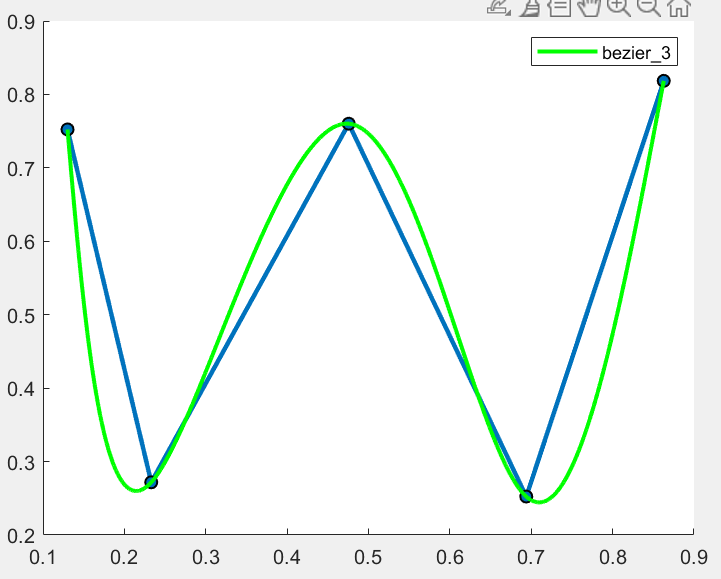
\includegraphics{w}
		\caption{}
		\label{fig:w}
	\end{figure}
	\begin{figure}[H]
		\centering
		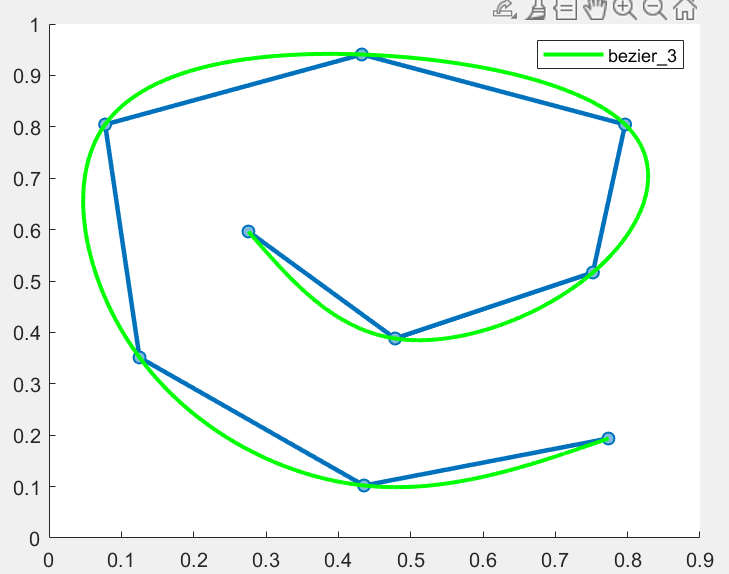
\includegraphics{e}
		\caption{}
		\label{fig:e}
	\end{figure}
	\begin{figure}[H]
		\centering
		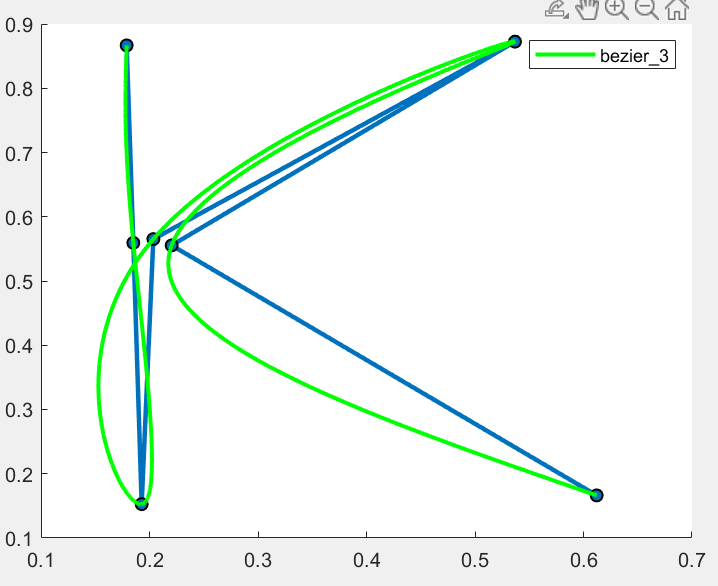
\includegraphics{k}
		\caption{}
		\label{fig:k}
	\end{figure}
\section{实验结果分析}
	实现了3阶\Bezier样条曲线插值。

	
	
	
	
	
	
	
\end{document}











